% Generated from ../supplementary.tex for Springer Nature submission-style compilation.
% Source of truth remains ../supplementary.tex and ../content/10-supplementary.tex.
\documentclass[pdflatex,sn-nature]{sn-jnl}

\usepackage[utf8]{inputenc}
\usepackage[T1]{fontenc}
\usepackage{graphicx}
\usepackage{booktabs}
\usepackage[htt]{hyphenat}
\usepackage{xurl}
\usepackage{amsmath}
\usepackage{amssymb}
\usepackage{longtable}
\usepackage{array}
\usepackage{caption}
\usepackage{float}
\usepackage{subcaption}
\usepackage{xcolor}
\usepackage{listings}
\usepackage[expansion=false]{microtype}
\usepackage{parskip}
\usepackage{seqsplit}
\usepackage{tcolorbox}
\tcbuselibrary{breakable}

\graphicspath{{../}{../../}}

\lstset{
  basicstyle=\small\ttfamily,
  breaklines=true,
  breakatwhitespace=false,
  frame=single,
  backgroundcolor=\color{gray!10},
  xleftmargin=1em,
  xrightmargin=1em,
}

\hypersetup{
  colorlinks=true,
  linkcolor=blue,
  urlcolor=blue,
  citecolor=blue,
}

\newcommand{\protocolstep}[2]{\par\medskip\noindent\textbf{#1 \textbar{} #2}\par}
\newcommand{\setupitem}[1]{\par\medskip\noindent\textbf{#1}\par}
\setcounter{secnumdepth}{0}
\raggedbottom

\renewcommand{\thesubsection}{\arabic{subsection}}
\providecommand{\benchmarkroot}{../..}

\begin{document}

\title{Supplementary Notes}

\maketitle

\providecommand{\benchmarkroot}{..}
\setcounter{subsection}{0}
\renewcommand{\thesubsection}{\arabic{subsection}}
\newcommand{\supplementarynote}[1]{%
  \refstepcounter{subsection}%
  \subsection*{Note \thesubsection: #1}%
  \addcontentsline{toc}{subsection}{Note \thesubsection: #1}%
}

\supplementarynote{Re-analysis of published datasets}
\label{supp:analysis-of-published-datasets}

To assess the applicability of DELT-Hit to previously published DEL selections, we re-analyzed two literature datasets distributed with the supporting material: the NF2 dataset reported by Favalli et al.\cite{favalli_stereoregiodefineddnaencoded_2021} and the Pure-DEL dataset reported in Science\cite{keller_highlypurednaencoded_2024}. All studies presented here are low- to medium-complexity libraries, and the expected runtime for re-analysis is therefore in line with the timing guidance given in the main protocol.

{\sloppy
The workflow is available on GitHub. The top-level supporting-material index in \path{supporting_material/README.md} links to the Favalli re-analysis folder (\path{supporting_material/experiments/favalli/}), which contains the execution script (\path{run.sh}) and step-by-step reproduction instructions. The corresponding comparison script (\path{supporting_material/experiments/favalli/compare_selections.py}) shifts the DELT-Hit \texttt{code\_0}/\texttt{code\_1} identifiers to the published 1-based numbering and then matches them to the \texttt{CodeA}/\texttt{CodeB} columns of the original evaluation table. In this way, the DELT-Hit re-analysis reproduces the published count table that was originally generated with the C++ evaluation workflow referenced in the study. An example selection excerpt is shown in Supplementary Table~\ref{tab:favalli-example}.

The Pure-DEL library was analyzed in the original study with a further-developed version of the same C++ analysis lineage. In our re-analysis, DELT-Hit was run from the original FASTQ files using \path{supporting_material/experiments/pure-del/run.sh}, and the resulting count tables were compared with the Zenodo-deposited selection tables using the comparison script \path{supporting_material/experiments/pure-del/compare_selections.py}. This script shifts DELT-Hit \texttt{code\_0}/\texttt{code\_1}/\texttt{code\_2} identifiers to the deposited 1-based numbering and matches them to the \texttt{Code1}/\texttt{Code2}/\texttt{Code3} columns in the original tables. Across the two lane-specific reruns, the deposited selection count tables are recovered exactly for the corresponding deposited outputs, showing that the published Pure-DEL counts can be reproduced directly from the original sequencing data within the DELT-Hit workflow. An example selection excerpt is shown in Supplementary Table~\ref{tab:puredel-example}.
\par}

\begin{table}[htbp]
\centering
\small
\caption{Top 10 rows from the Favalli selection \texttt{10\_2} comparison table.}
\label{tab:favalli-example}
\begin{tabular}{rrrrr}
\toprule
\textbf{code\_0} & \textbf{code\_1} & \textbf{legacy} & \textbf{delt} & \textbf{identical} \\
\midrule
268 & 278 & 62 & 62 & True \\
67 & 278 & 59 & 59 & True \\
67 & 60 & 53 & 53 & True \\
3 & 278 & 51 & 51 & True \\
268 & 60 & 49 & 49 & True \\
204 & 16 & 47 & 47 & True \\
67 & 304 & 43 & 43 & True \\
193 & 16 & 42 & 42 & True \\
67 & 230 & 42 & 42 & True \\
268 & 230 & 39 & 39 & True \\
\bottomrule
\end{tabular}
\end{table}

\begin{table}[htbp]
\centering
\small
\caption{Top 10 rows from the Pure-DEL selection \texttt{16\_2} comparison table.}
\label{tab:puredel-example}
\begin{tabular}{rrrrrr}
\toprule
\textbf{code\_0} & \textbf{code\_1} & \textbf{code\_2} & \textbf{legacy} & \textbf{delt} & \textbf{identical} \\
\midrule
9 & 1 & 11 & 82237 & 82237 & True \\
9 & 4 & 11 & 75428 & 75428 & True \\
9 & 5 & 11 & 69178 & 69178 & True \\
9 & 7 & 11 & 66951 & 66951 & True \\
8 & 10 & 11 & 63161 & 63161 & True \\
9 & 10 & 11 & 63147 & 63147 & True \\
9 & 8 & 11 & 58942 & 58942 & True \\
8 & 4 & 11 & 55386 & 55386 & True \\
8 & 7 & 11 & 53387 & 53387 & True \\
9 & 2 & 11 & 49307 & 49307 & True \\
\bottomrule
\end{tabular}
\end{table}

\supplementarynote{DELT-Hit and DELi workflow comparison}
\label{supp:comparison-delt-deli}

\providecommand{\statusgreen}{\raisebox{0.15ex}{\textcolor{green!50!black}{\LARGE$\bullet$}}}
\providecommand{\statusamber}{\raisebox{0.15ex}{\textcolor{orange!90!black}{\LARGE$\bullet$}}}
\providecommand{\statusopen}{\raisebox{0.15ex}{\textcolor{black!45}{\LARGE$\bullet$}}}
\providecommand{\statusred}{\raisebox{0.15ex}{\textcolor{blue!70!black}{\LARGE$\bullet$}}}

The main text summarizes the DELT-Hit--DELi\cite{wellnitz_opensourcednaencodedlibrary_2025} comparison as a compact status table organized by scientific-software criteria rather than by a flat feature checklist. This note provides the minimum context required to interpret those status assignments.

\subsubsection{Qualitative functionality}

\paragraph{Scoring scheme.}
The table uses a four-state legend. \statusgreen\ indicates direct and explicit support in the cited source. \statusamber\ indicates partial support, narrower scope, or a workflow that is present but less fully documented or less broadly integrated. \statusopen\ indicates that the capability was not clearly demonstrated in the cited source. \statusred\ indicates that the cited source explicitly frames the capability as absent or as future work. DELi scores in the main-text table are based only on the DELi preprint shared for this comparison; they are not inferred from external documentation or repository inspection.

\paragraph{1. Workflow scope and usability.}
DELi is scored \statusgreen\ for library design support because the preprint explicitly presents DELi as a platform for library design and describes a dedicated barcode-design module based on quaternary Hamming codes. For DELT-Hit, we assign \statusamber\ because this manuscript documents strong design-adjacent support through library specification, reaction-graph definition, enumeration, visualization, property calculation, and representation export, but does not present a dedicated barcode-design or library-design module. Both tools are scored \statusgreen\ for configuration and workflow ergonomics because both descriptions emphasize a coherent command-line workflow with structured human-editable configuration. We assign DELT-Hit \statusgreen\ for interoperability and downstream reuse because the manuscript and repository emphasize standardized tabular outputs, executable scripts, parquet exports, and downstream cheminformatics or machine-learning handoff. DELi is scored \statusamber\ because the preprint clearly supports modular reuse and export of decoded count tables, but describes downstream reuse less systematically than DELT-Hit and emphasizes internal report-generation and integrated analysis workflows more strongly.

\paragraph{2. Supported DEL architectures.}
Both frameworks are scored \statusgreen\ for single-display support because this capability is explicit in both sources. For DELT-Hit, we assign \statusgreen\ for dual-display support because the manuscript explicitly claims support for single-display and dual-display workflows, and the implementation includes dual-display configuration validation and dual-display enumeration logic. This score is intended at the workflow level; some downstream DELT-Hit utilities still assume a single \texttt{smiles} column and therefore do not yet cover every dual-display output path symmetrically. DELi is scored \statusopen\ for dual-display support because the preprint documents heterogeneous DEL decoding and general barcode flexibility, but does not explicitly describe a dual-display analysis workflow or claim dual-display support directly.

\paragraph{3. Decoding and sequencing-side QC.}
Both tools are scored \statusgreen\ for error-tolerant demultiplexing because both descriptions explicitly combine read-to-library assignment with configurable error-tolerant barcode handling. DELi is scored \statusgreen\ for UMI-aware counting because the preprint explicitly states that UMI-corrected counting is supported and stored alongside raw counts. For DELT-Hit, we assign \statusamber\ on this row because the workflow supports UMI-aware processing in a narrower and less prominently documented form than in DELi, rather than as a comparably explicit end-to-end feature. Both tools are scored \statusgreen\ for decoding QC and reporting, but the emphasis differs: DELT-Hit exposes text reports, QC plots, and an interactive count dashboard, whereas DELi emphasizes robust failure logging and configurable HTML reports.

\paragraph{4. Chemical reconstruction and enumeration.}
Both frameworks are scored \statusgreen\ for library enumeration because both sources explicitly document full-library enumeration from encoded building blocks and reaction definitions. For DELT-Hit, we assign \statusgreen\ for flexible reaction-scheme support because the manuscript explicitly describes an explicit reaction graph supporting arbitrary reaction sequences, branching pathways, and multi-step transformations, alongside visualization and debugging aids for failed enumerations. DELi is scored \statusred\ for this row because the preprint states that support for nonlinear and conditional synthesis schemes is planned for future updates, which makes the current scope narrower than the DELT-Hit workflow described in the manuscript.

\paragraph{5. Statistical analysis and hit interpretation.}
Both frameworks are scored \statusgreen\ for count-based enrichment because each tool supports compound-level ranking from decoded count data. Both are also scored \statusgreen\ for statistical enrichment scoring, but for different reasons. In DELT-Hit, the manuscript presents simple count-based analysis together with normalized z-score scoring and replicate-aware \texttt{edgeR} analysis, whereas DELi emphasizes a broader menu of literature-derived enrichment metrics. DELi is scored \statusgreen\ for synthon-level analysis because the preprint explicitly describes di- and monosynthon analysis and illustrates disynthon-level reporting. For DELT-Hit, we assign \statusred\ for this row because the manuscript and repository materials reviewed here do not document synthon-level analysis as a dedicated analysis mode.

\paragraph{6. Computational performance.}
For DELT-Hit, we assign \statusgreen\ for memory and scaling behavior because the manuscript provides explicit timing expectations across dataset scales, qualitative RAM guidance, and a workflow design that uses multiple CPU cores during demultiplexing and post-processing. DELi is scored \statusamber\ because the preprint reports single-core throughput and describes external Nextflow-based parallel deployment, but gives less explicit memory characterization and less detailed scaling guidance than DELT-Hit.

\subsubsection{Quantitative runtime and memory complexity}

\paragraph{Synthetic demultiplexing benchmark.}
To complement the workflow-level comparison above, we benchmarked DELT-Hit and
DELi (version 0.2.0, local checkout 8b8f8b5) on shared synthetic FASTQ
datasets designed to isolate demultiplexing performance under matched input
conditions. The benchmark covers canonical 2-, 3-, and 4-cycle libraries with
10 building blocks per cycle across 1M, 10M, 100M, and 1000M reads, and
additionally includes an extended 2-cycle sweep with 10, 100, and 1000
building blocks per cycle. Jobs were executed on a HPC Slurm cluster with 12
CPUs and 128\,GB RAM allocated per run. The reported outputs focus on
end-to-end runtime and peak RSS memory for the shared benchmark setup; the
DELi 1000M-read runs terminated in an out-of-memory state.

Supplementary Figure~\ref{fig:delt-deli-runtime-cycles} summarizes cycle-wise
runtime scaling, Supplementary Figure~\ref{fig:delt-deli-runtime-2cycle-bbpc}
shows the extended 2-cycle runtime sweep, and Supplementary
Figure~\ref{fig:delt-deli-memory-cycles} summarizes peak RSS scaling. Within
this benchmark setup, DELT-Hit is markedly superior to DELi in both runtime
and memory scaling. The gap is large enough that analysis at industry-relevant
library and sequencing scales is not practically feasible with DELi under the
tested conditions.

\begin{figure}[H]
\centering

\includegraphics[width=0.32\textwidth]{\benchmarkroot/benchmarks/demultiplex/plots/synthetic_2cycle_10bbpc_runtime.png}\hfill

\includegraphics[width=0.32\textwidth]{\benchmarkroot/benchmarks/demultiplex/plots/synthetic_3cycle_10bbpc_runtime.png}\hfill

\includegraphics[width=0.32\textwidth]{\benchmarkroot/benchmarks/demultiplex/plots/synthetic_4cycle_10bbpc_runtime.png}
\caption{Cycle-wise runtime scaling for the canonical synthetic demultiplex benchmark at 10 building blocks per cycle across 1M to 1000M reads. The DELi 1000M-read runs exited with an out-of-memory state.}
\label{fig:delt-deli-runtime-cycles}
\end{figure}

\begin{figure}[H]
\centering

\includegraphics[width=0.75\textwidth]{\benchmarkroot/benchmarks/demultiplex/plots/synthetic_2cycle_bbpc_comparison_runtime.png}
\caption{Runtime scaling for the extended 2-cycle synthetic benchmark across 10, 100, and 1000 building blocks per cycle.}
\label{fig:delt-deli-runtime-2cycle-bbpc}
\end{figure}

\begin{figure}[H]
\centering

\includegraphics[width=0.32\textwidth]{\benchmarkroot/benchmarks/demultiplex/plots/synthetic_2cycle_10bbpc_peak_rss.png}\hfill

\includegraphics[width=0.32\textwidth]{\benchmarkroot/benchmarks/demultiplex/plots/synthetic_3cycle_10bbpc_peak_rss.png}\hfill

\includegraphics[width=0.32\textwidth]{\benchmarkroot/benchmarks/demultiplex/plots/synthetic_4cycle_10bbpc_peak_rss.png}
\caption{Peak memory usage (RSS) per cycle for the canonical synthetic demultiplex benchmark (10 building blocks per cycle), evaluated from 1 million to 1 billion reads. The DELi runs at 1 billion reads terminated due to out-of-memory (OOM).}
\label{fig:delt-deli-memory-cycles}
\end{figure}

\supplementarynote{Enrichment Scores}
\label{supp:enrichment-scores}

This section defines the DELT-Hit enrichment methods and the experimental
settings where each is most appropriate.

\textbf{Count Method.}
The count method averages raw sequencing counts across replicates within each
group and scores each compound by the difference between the condition
and control means, $\bar{c}_{\rm cond} - \bar{c}_{\rm ctrl}$. It is a
transparent count-based baseline that averages replicate counts and does not
assume a parametric count distribution. Its main weakness is sensitivity to
read-depth differences and raw-count scale, because the current default workflow
operates on raw counts rather than library-size-normalized frequencies. It is
therefore most informative when sequencing depths are comparable or as a simple
benchmark baseline.

\textbf{Z-Score Method (Faver et al.\ formulation).}
Let $D$ denote the total number of distinct disynthon (or higher-cycle) compound
identities in the library and $n$ the total number of sequencing reads in a
selection. For a given compound, let $c$ be its raw read count. The observed
sequence frequency is $p_{\rm obs} = c / n$ and the expected null frequency under
uniform library representation is $p_i = 1/D$. The depth-insensitive z-score
is\cite{faver_quantitativecomparisonenrichment_2019}

\begin{equation}
z_n = \frac{p_{\rm obs} - p_i}{\sqrt{p_i\,(1 - p_i)}}.
\label{eq:zscore}
\end{equation}

The closely related fold enrichment,
\begin{equation}
E = \frac{p_{\rm obs}}{p_i} = c \cdot \frac{D}{n},
\label{eq:fe}
\end{equation}
provides a scale-invariant measure of enrichment that is more interpretable for
hit-picking. Equations~\ref{eq:zscore} and \ref{eq:fe} summarize these two
related views. The recommended primary hit threshold is $E \geq 2.0$; a fixed
$z_n$ cutoff is not recommended because practical score ranges depend on
library diversity, sampling sparsity, and selection context.

\textbf{edgeR Method.}
Compound-level read counts per selection are modelled as negative-binomial
(NB) random variables. The NB model accommodates overdispersion relative to
Poisson counts, which arises in DEL experiments from variation in sequencing
depth, barcode-decoding efficiency, and chemical synthesis yield. Per-compound
dispersion is estimated by empirical Bayes shrinkage towards a trend fitted
across all compounds\cite{robinson_edgerbioconductorpackage_2010}. A likelihood-ratio test (LRT) is performed
for each compound to compare the NB-GLM fit under a two-group design
(condition vs.\ control) against a null model; Benjamini--Hochberg
false-discovery rate (FDR) correction is applied across all compounds.
Compounds are ranked by log$_2$ fold change (logFC); FDR is available as a
secondary filter.

\supplementarynote{Comparison of enrichment score rankings for the Favalli CAIX selection}
\label{supp:enrichment-scores-comparison}

To compare the ranking schemes implemented in DELT-Hit, we re-analyzed the Favalli selection against CAIX. As a
literature-supported positive-control motif, we focused on building block 1, code 474, which occurs in previously
reported CAIX-binding compounds from related DEL selections\cite{bassi_singlestrandeddnaencodedchemical_2020,favalli_stereoregiodefineddnaencoded_2021}. For the count-based and edgeR analyses, compounds were ordered by the corresponding aggregate score, and the occurrence of building block 1/code 474 was counted among the top 10, 25, 50, and 100 ranked compounds. Because the z-score method is computed at the individual-selection level, compounds were ranked separately for each replicate, the occurrence of code 474 was counted independently within each replicate-specific top list, and the bar plot reports the mean with the replicate standard deviation. This recovery analysis provides a high-level comparison of how effectively the different ranking strategies prioritize a known CAIX-associated building block. The analysis indicates that the edgeR-based methods are more sensitive than pure count-based ranking. The top-50 recovery comparison is summarized in Supplementary Figure~\ref{fig:favalli-ca9-ds-top50-code1}. Scripts to reproduce the analysis are described in \path{supporting_material/experiments/favalli/README.md}.

\begin{figure}[htbp]
\centering
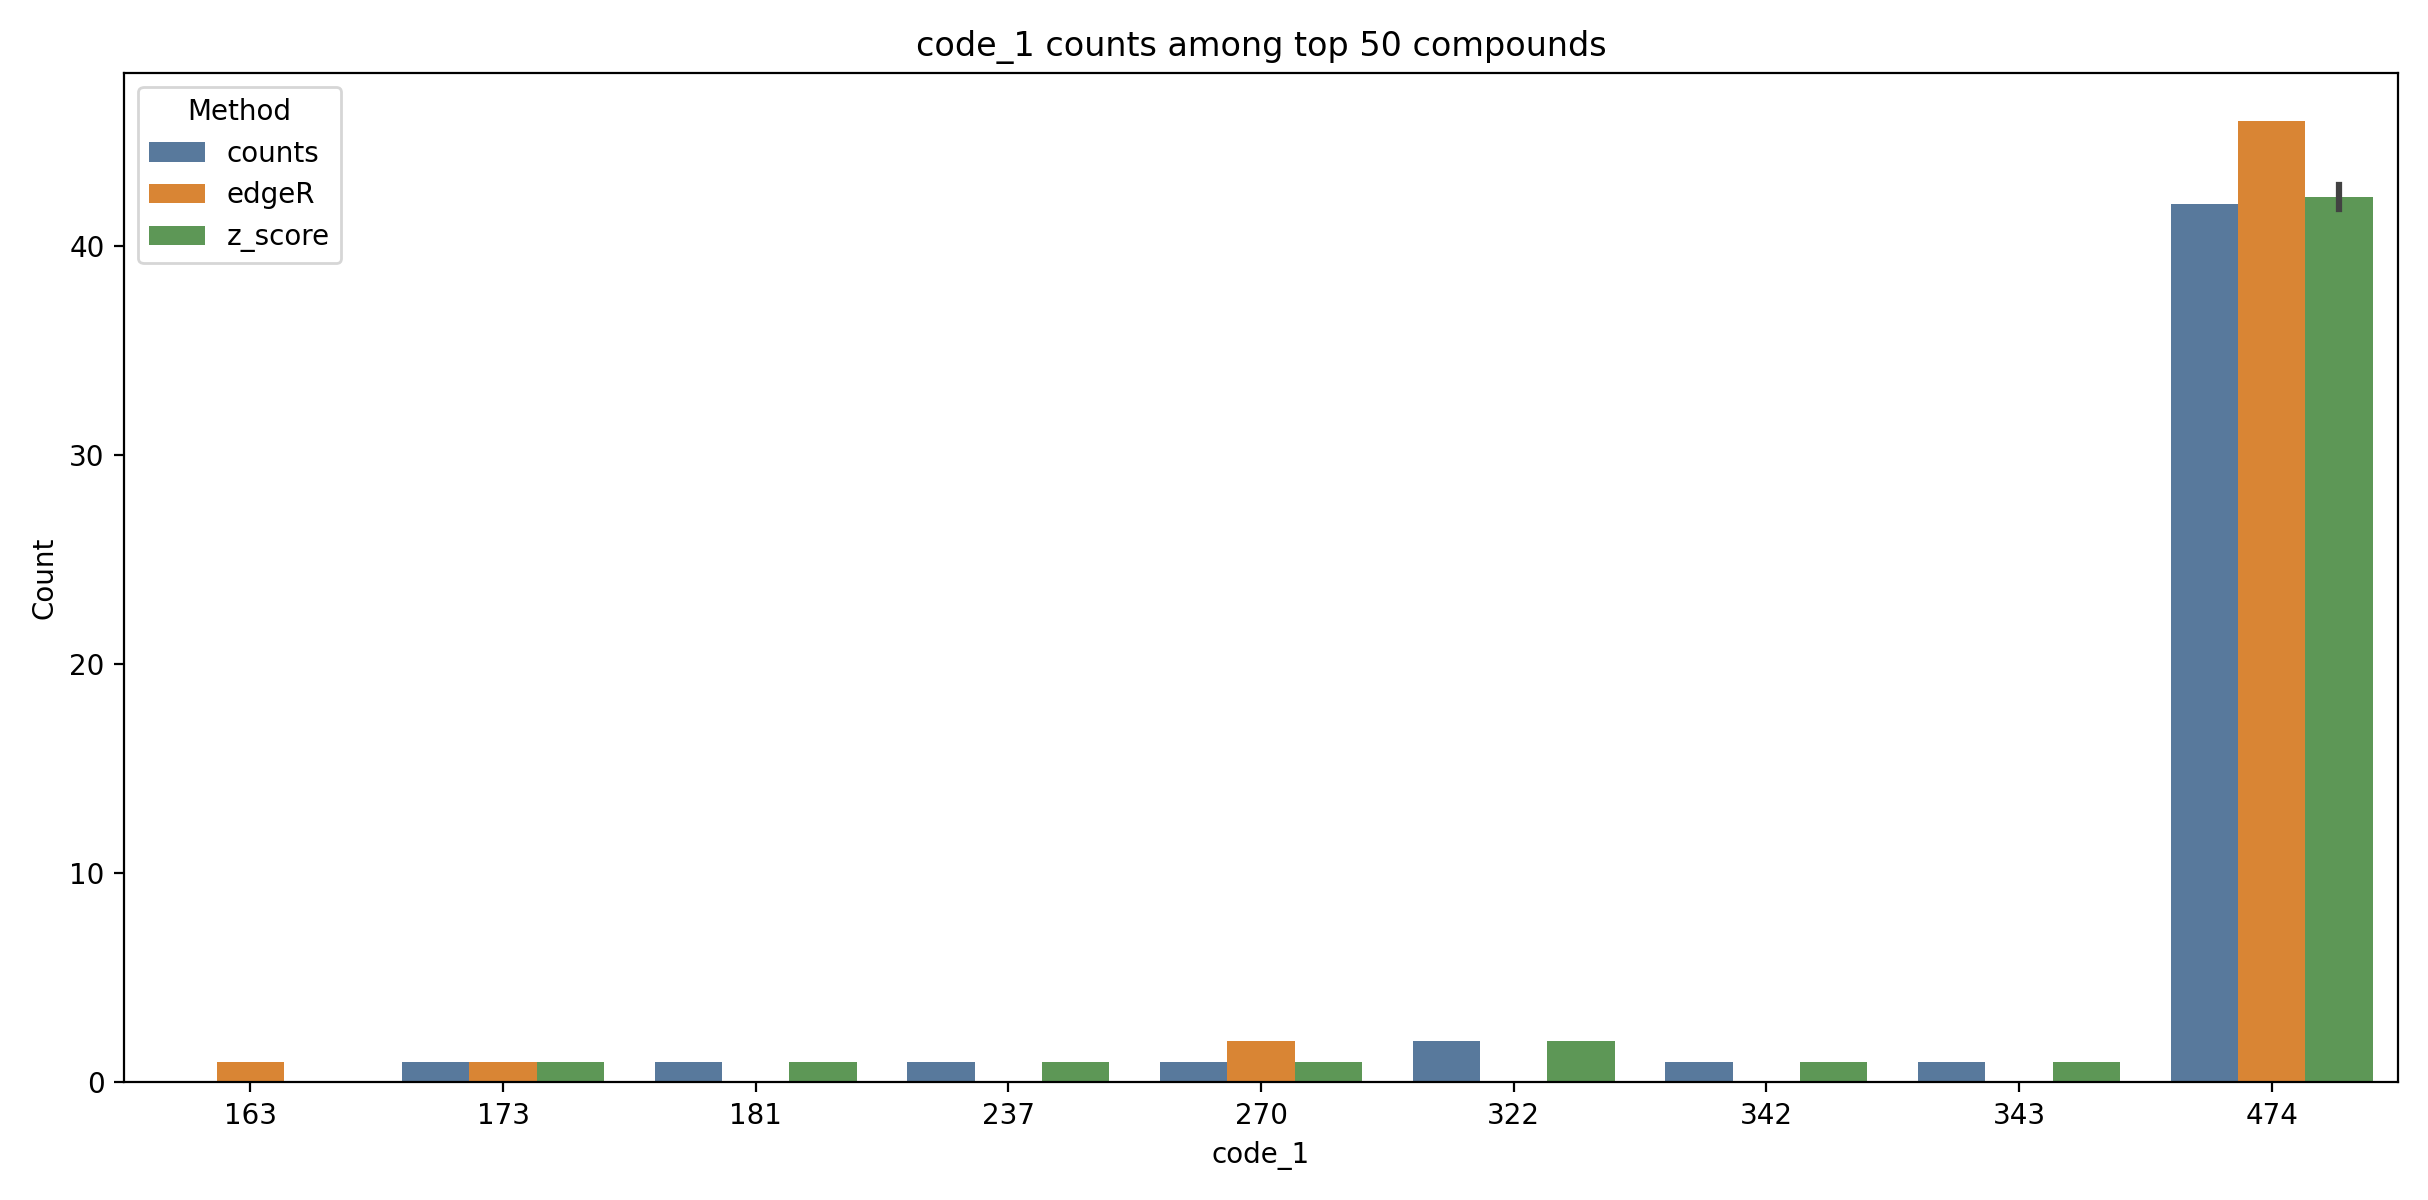
\includegraphics[width=0.9\linewidth]{figures/supp-favalli-ca9-top50-code1-counts.png}
\caption{Occurrence counts of code 1 building blocks among the top 50 ranked compounds for the Favalli CAIX selection analysis. For the z-score method, bars show the mean across replicate-specific top-50 selections and the error bars show the replicate standard deviation.}
\label{fig:favalli-ca9-ds-top50-code1}
\end{figure}

\supplementarynote{Advanced reaction-graph configurations}
\label{supp:reaction-graph-advanced}

In the single-display tutorial workflow used in the main protocol, the only additional reaction-graph step is an \texttt{SR} transformation from \texttt{product\_1} to \texttt{product\_1B}, represented in the \texttt{reaction\_graph} sheet by the row \texttt{product\_1, , SR, product\_1B}. More advanced library designs can require multiple precursor-activation paths even when they conceptually share the same transformation class.

For example, two scaffolds that both require Staudinger reduction before entering subsequent coupling steps should be encoded as separate reaction paths in the \texttt{reaction\_graph} sheet, as summarized in Supplementary Table~\ref{tab:table11}:

% BEGIN flattened input: tables/precursor-activation-reactions
\begin{table}[htbp]
\centering
\caption{Additional reaction step definitions (special case)}
\label{tab:table11}
\begin{tabular}{llll}
\toprule
educt\_1 & educt\_2 & reaction & product \\
\midrule
scaffold\_1 &  & SR\_precursor\_1 & scaffold\_1B \\
scaffold\_2 &  & SR\_precursor\_2 & scaffold\_2B \\
\bottomrule
\end{tabular}
\end{table}
% END flattened input: tables/precursor-activation-reactions
This explicit encoding keeps the reaction graph resolvable as independent paths. In contrast, reusing the same reaction node for both precursor activations would create an ambiguous graph assignment.

\bibliography{../zotero}

\end{document}
